\documentclass[a4paper,12pt]{report}

\setcounter{tocdepth}{3}
\setcounter{secnumdepth}{3}
\usepackage{graphicx}   %Package helps to insert images
\usepackage{times}
\usepackage{hyperref}

\begin{document}
\pagenumbering{roman}
%\usepackage[T1]{fontenc} 

%#################################
\begin{titlepage}
   \begin{center}
       \vspace*{1cm}

       \textbf{\large {\bf KANTIPUR ENGINEERING COLLAGE
                       DHAPAKHEL,LALITPUR} }
                       
                       %%College Logo                      
        \begin{figure}[htb!]
              \centering
              
\includegraphics[width=2.5cm, height=2.4cm]{images/ClzLogo.png} 
        \end{figure}
        
        \hspace{0.5cm}
       \textbf{\small{ [ Subject Code: CT654] }}\\
     {\bf MINOR PROJECT REPORT ON \\ BLOCKCHAIN BASED ONLINE VOTING SYSTEM FOR COLLEGE LEVEL ELECTIONS }
     
       \vspace{2.3cm}
    \textbf{\small
                Submitted By:\\
                Bijaya Thebe   [KAN076BCT018] \\
                Binit Shakya    [KAN076BCT022] \\
                Dikshyanta Giri [KAN076BCT026] \\
                Nawaraj Shah [KAN076BCT044] \\
                }


        \vspace{2cm}
         \textbf{\small{IN PARTIAL FULFILLMENT OF THE REQUIREMENT 
         FOR THE DEGREE OF  BACHELOR IN COMPUTER ENGINEERING}}
            
            
       \vspace{1.5cm}

%       \setromanfont{Times New Roman}

       \vfill
            
       \vspace{0.8cm}
            
       \textbf{\small
           Submitted To:\\
           Department of Computer and Electronics Engineering
           }
           
           \vfill
       \vspace{0.5cm}
         \textbf{\small  Jan 1 ,2023}
            
   \end{center}
\end{titlepage}

%#################################

\chapter*{Abstract}
In a democracy, elections are very important. However, large sections of society worldwide, people, and the government face various problems, including privacy, fairness, flexibility, and transparency of the voting system. So the government and people with the expertise move toward an electronic voting system. It provides flexibility to the different parties like commissions and people. However, privacy and security cannot be guaranteed in the Electronic Voting System, due to which the fairness and transparency won’t get as expected. This problem translates to college level elections as well. This paper proposed the Blockchain-Based Online Voting System, which can be a sound solution for maintaining privacy and fairness. It provides a decentralized database keeping system, an advanced  existing system that provides security and maintains the privacy of voters and commissions. So the trust of flexibility, as well as transparency, can be comfortably maintained with fewer amounts of effort.
\\
\textit{Keywords - Blockchain, Voting, Security, Transparent}
\chapter*{Acknowledgment}
The completion of this case study could not have been possible without the participation and assistance of various individuals. Foremost, We would  like to thank our computer project coordinator Er. Bishal Thapa for providing us with this opportunity.  We are also thank to our seniors - Anisha Rai and Grishan Pradhan who already work on blockchain project, and share their experience which help a lot to guide our project. Also, We would like to place many thanks to the Department of Computer and Electronics Engineering Department and Head of Department Er. Rabindra Khati for accepting our request and supporting us in this endeavor. Lastly, we are thankful for all who have helped us directly and indirectly.\\
Bijaya Thebe\\
Binit Shakya\\
Dikshyanta Giri\\
Nawaraj Shah

\renewcommand*\contentsname{Table of Contents}
\tableofcontents


\newpage

\pagenumbering{arabic}

\chapter{Introduction}

\section{Background}
Voting has always been an integral part of a democracy.  Voting is the ultimate right that can be utilized in a Democracy.  There  have been witnessed so many voting methods in our history, from holding up hands in an assembly in the ancient Greek era to paper ballots and electronic voting machines.

A paper-based voting system where voters use paper to cast a vote by stamping on their chosen candidate. This system has been used for a long time and is almost obsolete in many countries. Many countries use electronic voting systems as the main voting system. In this system, voters vote by pressing a button of their choice. However, no matter the system, the voting location has never been changed.

An online voting system is an online voting technique. In this system, people whom the admin authorizes can cast their vote online without going to any physical polling station.
 
In our country, Nepal, where many people cannot vote because they are far from their homes, this is also one of the main causes for fewer people to vote in elections. Our voting system helps to minimize this problem, as people can vote using a simple mobile phone or laptop/Computer from anywhere, which will help more people participate in the election. 
 
Also in college level elections, students will be more willing to vote if  they are provided with an easy alternative to physical voting.

\section{Problem Statement}
Voting is considered a very important aspect of any democratic country. 
As important as it is, it is also very hard to conduct a perfect election. Problems may arise due to various aspects. Most of the problems are caused intentionally, like rigging the votes, unregistered voters casting votes, and casting votes in place of others. However, recently the world faced an even bigger problem Covid-19 pandemic which shows the disadvantages of physical voting.

Due to the pandemic, many people tend to stay home rather than go to polling booths to cast their votes, which has made us realize the problem of the location of elections. Moreover, In the electronic voting system, the main problem is using the internet to transfer data to the server, which faces a huge risk of hacking and manipulating data. 
Also in college level elections there is a similar problem where the students would rather stay at home than to participate in the voting process.

\section{Objectives}
The main objectives of this application are mentioned below:\\
1. To make an Immutable voting system.\\
2. To provide a decentralized \\
3. Environment for voting.\\
4. To allow the eligible users to vote remotely.

\section{Application Scope}
This application is a blockchain-based voting system. Users use this web application to give their valuable votes to the right candidate. The primary purpose of this application is for the college level elections. However, this application can be modified for other voting systems.

\section{Project Feature}
The application is targeted toward the general population. So the features of this application can be listed below:\\
1. Voters Verifiability\\
2. Recoverability and Identification\\
3. Accessibility and Reassurance\\
4. Availability and Mobility\\
5. Transparency and Fairness\\
6. Vote Privacy\\
7. Democracy/Singularity

\section{System Requirements}
The development of any application needs some basic requirements. On this basis, this paper classified the requirements into two categories:

\subsection{Development Requirements}
Development requirements mainly focus on and imply only the building-up of the application blocks. So for developing this E-Voting app, some requirements are needed for carrying out the different tasks. It is broadly classified into two categories:

\subsubsection{Hardware Requirements}
Since this application is specifically focused on a specific task, i.e., is E-Voting. So for this, feasible and compatible devices are required. They are listed below:-\\
1. Intel Core - i5 processors (.i.e., Validated I-Series Processor or more) with a minimum of 4 G.B. RAM for applicational operation.\\
2. Server With optimal node speed  

\subsubsection{Software Requirements}
The application is targeted at specific and only authorized users. So It is aimed to be fully secured and optimized for carried out from intermediate to High-Range Systems. So we emphasize security and why the Blockchain technology system can be used. The list includes the following resources:-\\
1. Operating Systems: Windows 10 or Above\\
2. Web Technologies/Programming Language: HTML, CSS, Javascript, React, Solidity, Nodejs\\
3. Visual Studio Code

\subsection{Deployment Requirements}
Deployment is how applications, modules, updates, and patches are delivered from developers to users. So it needs some well-paved path to deploy it. Here users might be authorized as well as public people. Some requirements are listed below:-\\
1. Network-Communities: Ethereum network and community\\
2. OTP Service


\section{Feasibility Study}


\subsection{Economic Feasibility}
There will be no charge for developing the application.  
 
\subsection{Technical Feasibility}
Technically, the system is feasible enough for most users, but a basic familiarity with web-based applications is expected from the users.

\subsection{Operational Feasibility}
The user does not need to be an expert in using web-based programs for the system's operation. People with a basic knowledge of web-based applications can use this application.

\subsection{Schedule Feasibility}
Scheduling defines the time allotted to each specified aspect of the project like designing, coding, testing, etc. Also, scheduling helps properly define and allocate the project's resources. Without proper scheduling, the project will likely encounter multiple issues throughout its development.
 
  \begin{figure}[htb!]
          \centering
           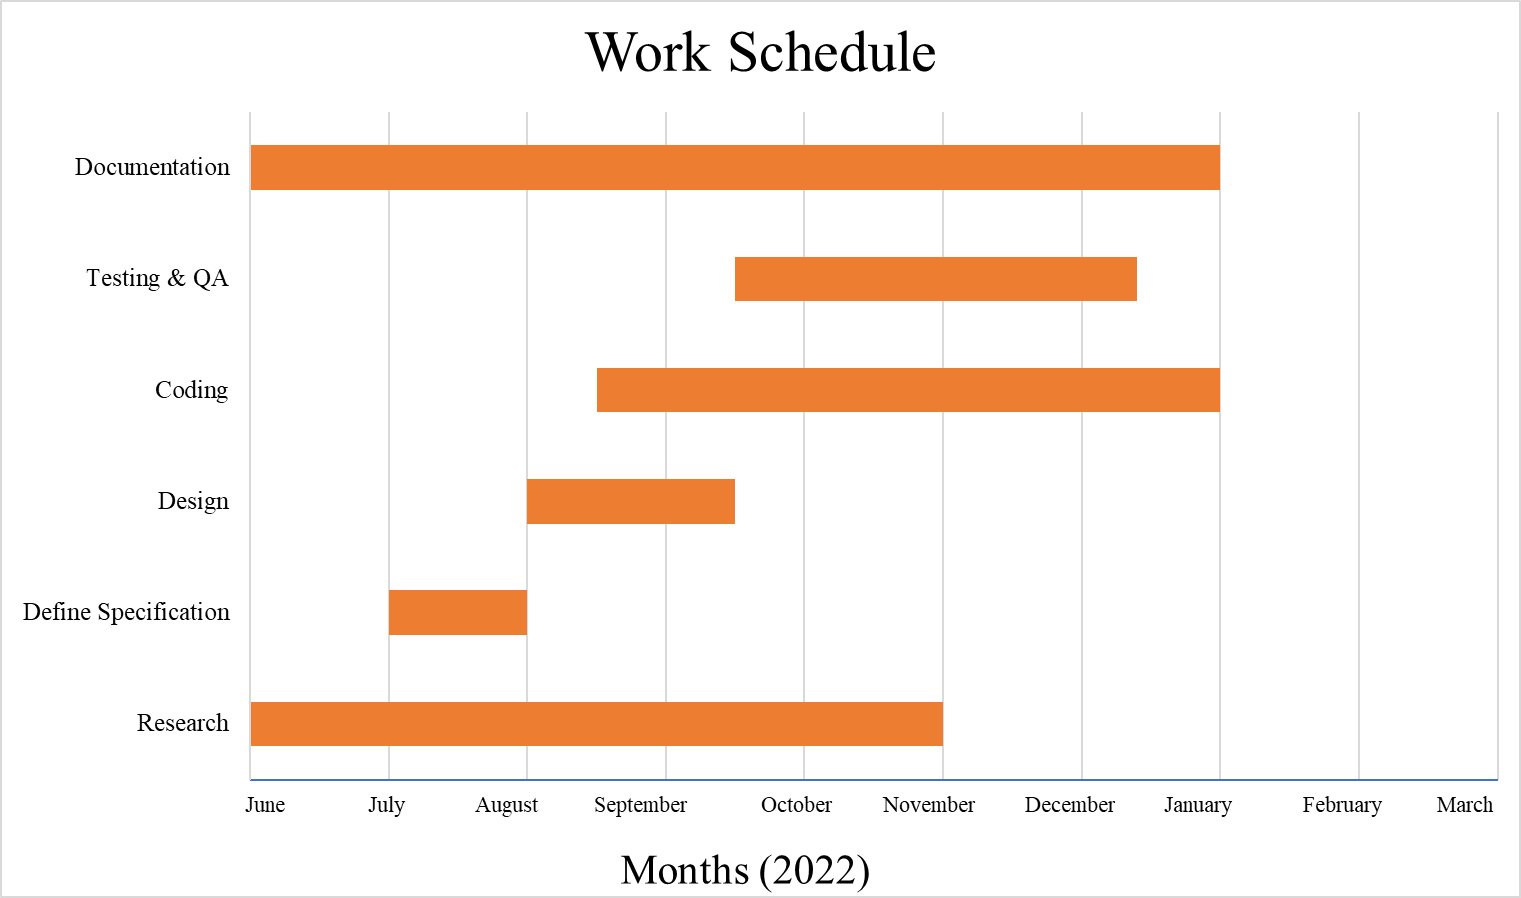
\includegraphics[scale=0.5]{images/GanttChat.png}     
          \textit{\caption{Gantt Chart of Working Schedule}}
          %\label{fig:BlockDiagram}
    \end{figure}


\chapter{LITERATURE REVIEW}
\section{Related Works}
An electronic voting system is essential for security and to protect the secrecy of a ballot, a core principle of fair and free elections. Block-chain offers a platform for creating a highly secure, anonymous, decentralized chain of records.

Moreover, free and fair elections are the bedrock of a democratic state. This is the essence of a block-chain-based voting system, making it difficult for external agents to tamper with it. This way, the voters can submit their votes without exposing their identity or political preferences to the public. In addition, the officials can count the votes with certainty that each identifier represents one vote while ensuring that fakes cannot be created and deliver a tamper-proof electoral process.

Due to these factors, many companies have emerged to develop electronic and blockchain-based voting systems. Some of the organizations include

\subsection{BallotReady}
BallotReady is an online, non-partisan voter guide for local elections. This is a system in which the users can look up their registration, plan to vote, and research the names on the ballot to prepare them before the voting process. This company focuses on educating the voters about everything necessary for voting.

\subsection{Voatz}
Voatz is a mobile Internet voting application that uses bio-metrics and block-chain to verify voters' identities and store the information in a database. Voatz application has already been used to cast ballots in the 2018 West Virginia elections, the 2016 Massachusetts Democratic State Convention, and a Philippines Trial Election.

\subsection{FollowMyVote}
FollowMyVote is an American organization aiming to make online voting easier, more secure, and cost-effective. The company aims to use block-chain technology and elliptic curve cryptography to make the voting process viable even online.

\section{Related Research}
There has been extensive research on adopting block-chain technology into online voting systems. Many research papers have been published on this subject. Some of the research papers were read during the research phase of our project.

\subsection{Blockchain}
Haber and Stornetta initially proposed the block-chain concept in 1991. Block-chain is a chain of blocks, which are time-stamped and linked cryptographic hashes. The block-chain is a distributed ledger of transactions carried out directly between consumers and providers on the system. A distributed network of nodes that preserve a common source of transactions. The nodes validate these transactions. Therefore the block-chain allows the creation of trust without a central authority.

Block-chain represents a means of recording and verifying documents transparently distributed among users of a selected network. Furthermore, votes should also be recorded, organized, counted, and verified for results to be published; this would eliminate illegitimate votes because the copies of the voter's voting history are recorded and can not be changed. Those changes can be easily verified.

This paper gives us an introduction to how the block-chain can be implemented in an e-voting system. This paper tackles the problems faced in the traditional system. By utilizing block-chain technology as a service in an e-voting system. Making a public block-chain platform provides immutability and transparency of the votes cast. This paper also gives us the advantages of using smart contracts to do various activities. Registering voters, Election creation, Tallying results, and Verifying votes are all guided by smart contracts, enabling faster, with less manpower, and secure form of election.

In another paper, they carried out the implementation of block-chain technology using the Ethereum platform. The main contribution of this paper is that they have proposed a message authentication and transmission mechanism that allows permission checking while preserving anonymity; this mechanism can be especially utilized in keeping the voter anonymous. The blind signing and checking procedure is also implemented, which helps authenticate the voters. And lastly, being based on Ethereum, it provides trusted computing technology and integrity to all parties involved.

Lastly, this paper gives an overview of how block-chain is implemented in an online voting system with the connection to the front-end; all in all, what a full-fledged dApp looks like. Using the Ethereum platform, the code for the application is written in a smart contract. The smart contract is logic that controls the flow of the application. Which also acts as a back-end for the decentralized application(dApp). So, the back-end is a block-chain that ensures that votes are counted and stored in a decentralized database, and the correct candidate with the most votes will win the election.

\chapter{METHODOLOGY}

\subsection{Block Diagram}
A block diagram is a drawing illustration of a system whose parts are illustrated by blocks. These blocks are joined by lines to display the relationship between the blocks. Block diagrams are used to visualize the functionality of a system.
   
    \begin{figure}[htb!]
          \centering
          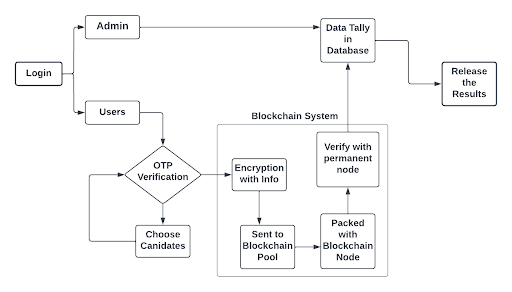
\includegraphics[scale=1]{images/BlockDig.png}  
          \textit{\caption{Block Diagram of Blockchain Online Voting System}}
          %\label{fig:BlockDiagram}
    \end{figure}

\paragraph{OTP Verification}
The system send OTP code to the verified user email address and that code is enter by the user and verified themselves.

\paragraph{Choose Candidate}
After users logged in to the system they enter into the select candidate page. There the user cast their vote to the respective candidate and again entering an updated OTP that he receives on his email address confirm the final process of voting. At third those information at the pool was packed into a Block-chain node which was created with the Keccak -256 Algorithm. At last node is finally verified with permanent node.With these four different steps the Block-chain system is carried out then proceeds to further steps.

\paragraph{Tally at Database}
The results are then tally at Database where the individual votes were recorded for individual candidate.The admin can control over the database for security purpose and initial monitoring of results but admin can't modify it on database.

\paragraph{Release Result}
Then at last the tally votes were shown in results which is done after all the process completion.

\paragraph{Nonce}
Nonce is the value used to calculate a block hash that meets a certain requirement.( Eg:- Start with a certain number of Zeroes).

\paragraph{Voting Data}
In this part of the block data is stored. Here the data about the voter count for candidate, whether the voter has already voted or not  and who the 
In this part of the block data is stored. Here data is divided to 2 parts one for the voter and one for the candidate. In the voter part the details about the voter are stored. It stores the data whether the voter has voted or not and which address the voter has voted for. In the candidate part it stores the name, address and total vote count of the candidate.

\paragraph{Previous Hash}
It is the hash of the block before it.It is used to link to the previous block.

\paragraph{Current Hash}
It is the hash ( .i.e.Hash is a unique fixed sized output for an input generated through a one way function called hash function) of the current data.

\section{System Models}
\subsection{Use Case Diagram}
A use case diagram is a way to summarize the details of a system and the users within that system. It is generally shown as a graphic depiction of interactions among different elements in a system. Use Case Diagrams will specify the events in a system and how those events flow. However, Use Case Diagram does not describe how those events are implemented.\\

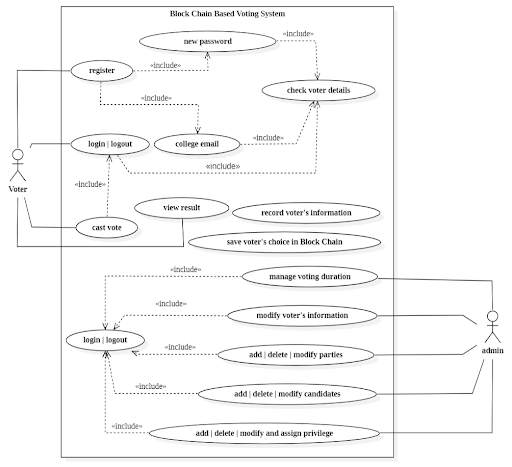
\includegraphics[scale=0.5]{images/UseCaseDig.png} 

\subsection{Data Flow Diagrams (DFD)}
In Software engineering, DFD(data flow diagram) can be drawn to represent the system of different levels of abstraction. Higher-level DFDs are partitioned into low levels-hacking more information and functional elements. Levels in DFD are numbered 0, 1, 2, or beyond. Here, we will see 2 levels in the data flow diagram: 0-level DFD and 1-level DFD.
\paragraph{0-level DFD}
It is also known as a context diagram. It is designed to be an abstraction view, showing the system as a single process related to external entities. It represents the entire system as a single bubble with input and output data indicated by incoming/outgoing arrows.

           \begin{figure}[htb!]
               \centering
               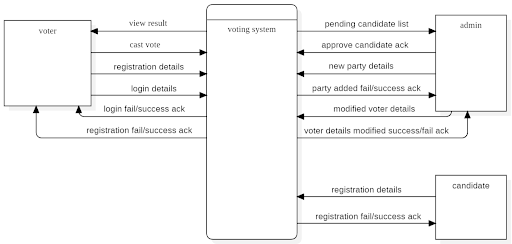
\includegraphics[scale=0.5]{images/DFD-0L.png} \\
               \textit{\caption{0-level data flow diagram}}
              % \label{fig:DFD Diagram 1}
         \end{figure}

\paragraph{1-level DFD}
In 1-level DFD, the context diagram is decomposed into multiple bubbles/processes. In this level, this report highlight the system's main functions and break down the high-level process of 0-level DFD into sub-processes.

     \begin{figure}[htb!]
               \centering
      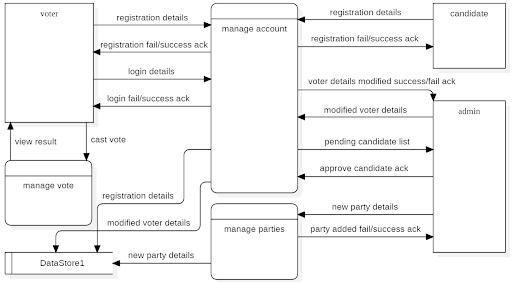
\includegraphics[scale=0.5]{images/DFD-1L.png} \\
               \textit{\caption{1-level data flow diagram}}
              % \label{fig:DFD Diagram 2}
         \end{figure}

\subsection{Activity diagram}
An activity diagram is a flowchart representing the flow from one activity to another. The activity can be described as an operation of the system.\\

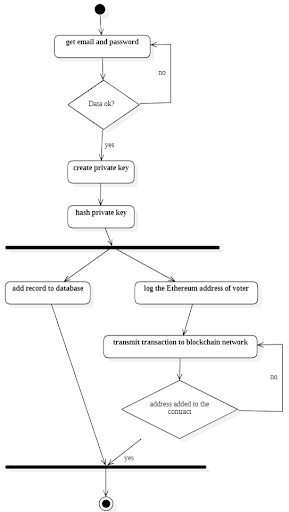
\includegraphics[scale=0.5]{images/ActivityDig-1.png}

\includegraphics[scale=0.5]{images/ActivityDig-2.png}
  
    %\begin{figure}
              % \centering
         %     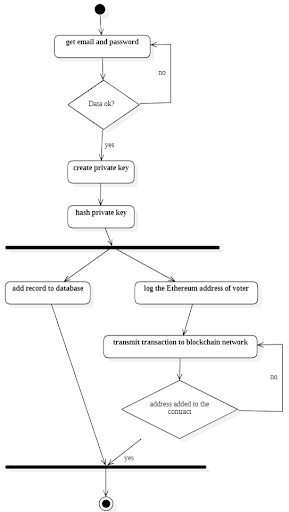
\includegraphics[scale=1]{images/ActivityDig-1.png} 
              % \textit{\caption{Activity Diagram for Registeration.}}
               
%             \includegraphics[scale=0.5]{ActivityDig-2}
                 % \textit{\caption{Activity Diagram for Voting.}}
             %  \label{fig:Activity Diagram 1}
        % \end{figure}

\subsection{Incremental Model}
The incremental model is a process of software development where requirements are divided into multiple standalone modules of the software development cycle. The incremental process model is also known as the Successive version model. This model emphasizes the full phase dynamic growing software. Since the E-voting software of our project is also a kind of dynamic software that needs the continuous development and full phase growth of different features like login portals, Conformation Portals, Voting Selection Portals, etc.\\

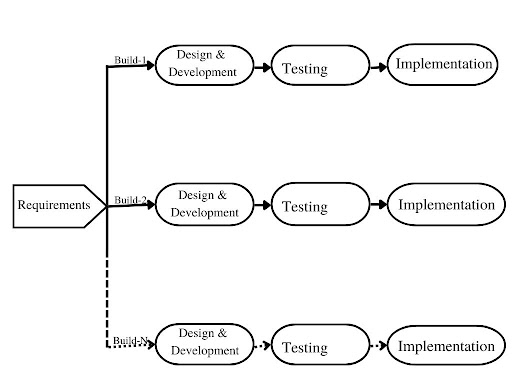
\includegraphics[scale=0.5]{images/DevModel.jpg} 

Incremental Models include the different building phases. Like Build-1, Build-2, Build-3……to……Build-N phases, where build ‘N’ is the defined possible steps.
\begin{itemize}
  \item Build-1: Login
  \item Build-2: API
  \item Build-3: Solidity Contracts
  \item Build-4: Acquire Voting from Voters
\end{itemize}
\chapter{EPILOGUE}

\subsection{Login and Verification}
 %\begin{figure}[!]
             % \centering
               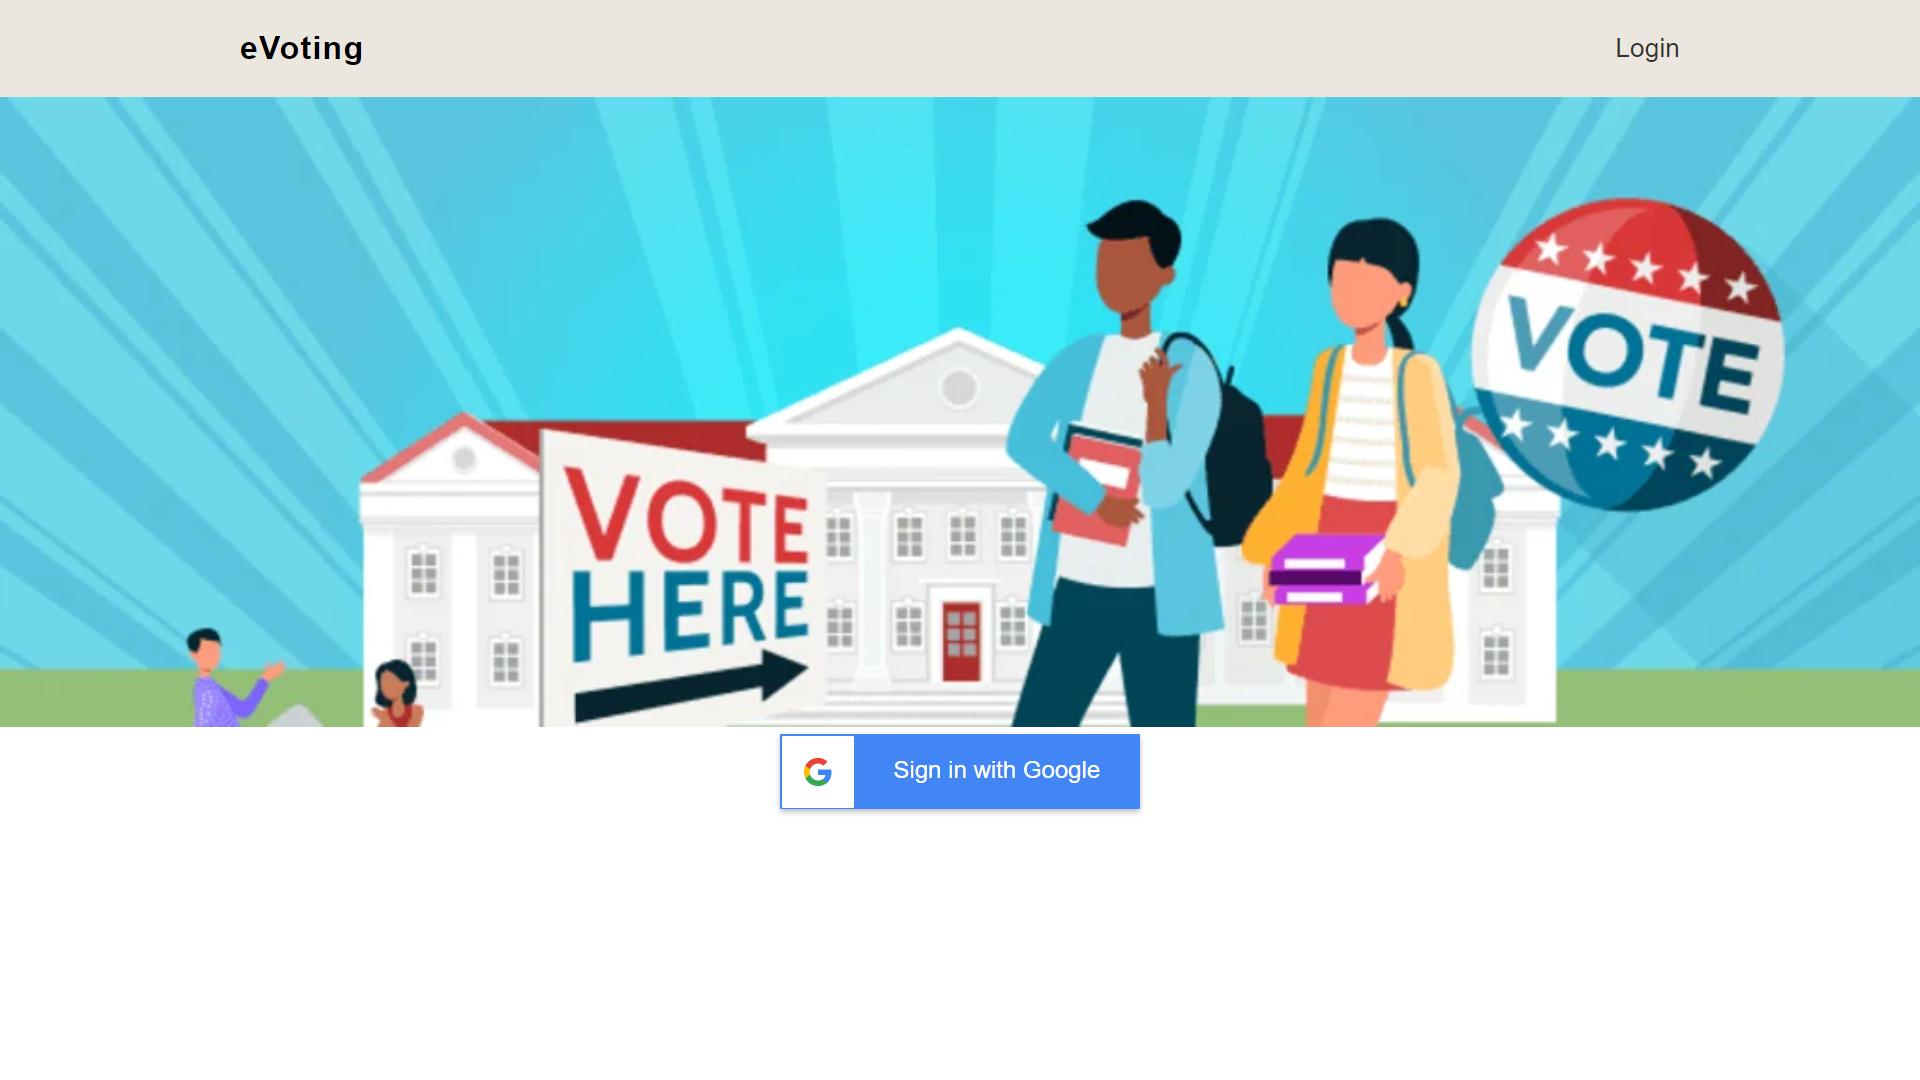
\includegraphics[scale=0.25]{images/Epilog-2.png} 
              % \textit{\caption{Login with Google.}}
               
                  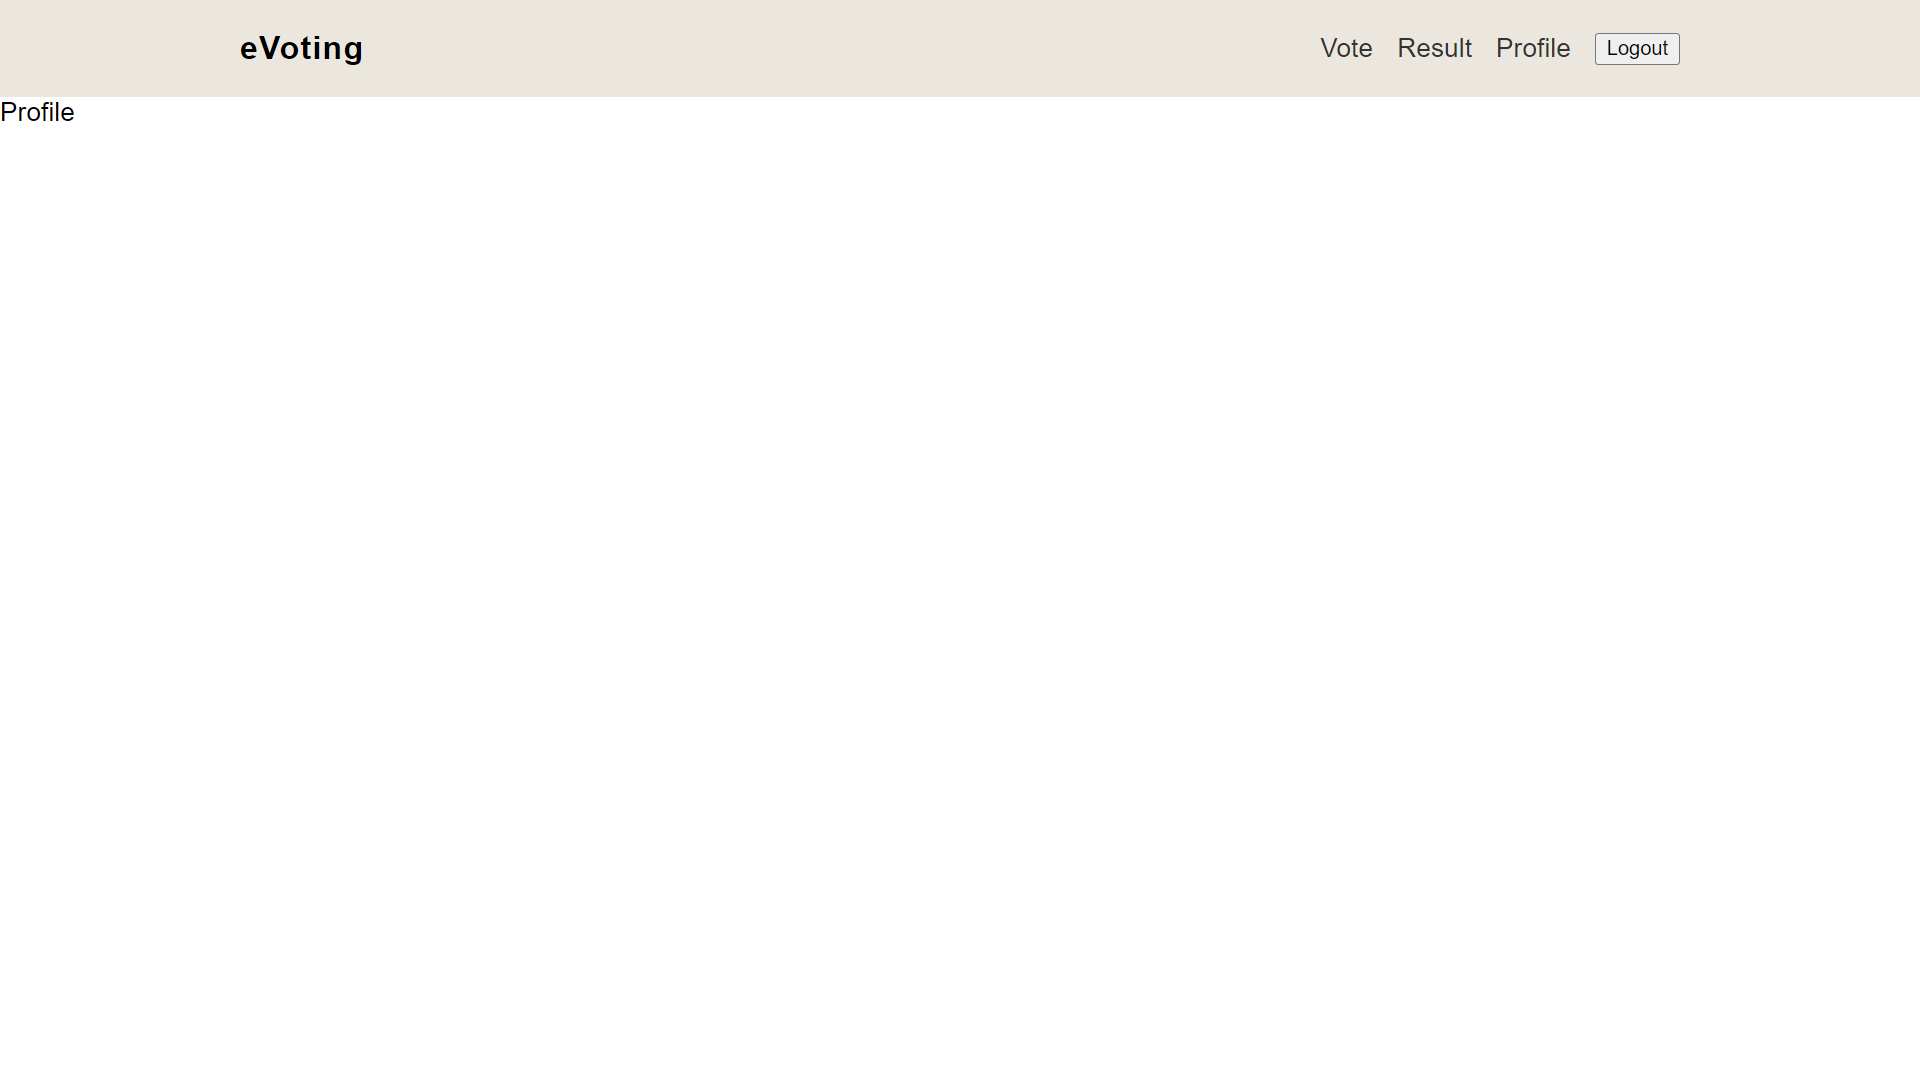
\includegraphics[scale=0.25]{images/Epilog-1.png} 
                  %\textit{\caption{Evoting Home Profile.}}
               
              % \label{fig:Activity Diagram 1}
       %  \end{figure}
         
         
\subsection{Smart Contract Output}
%\begin{figure}[!]
          %  \centering
      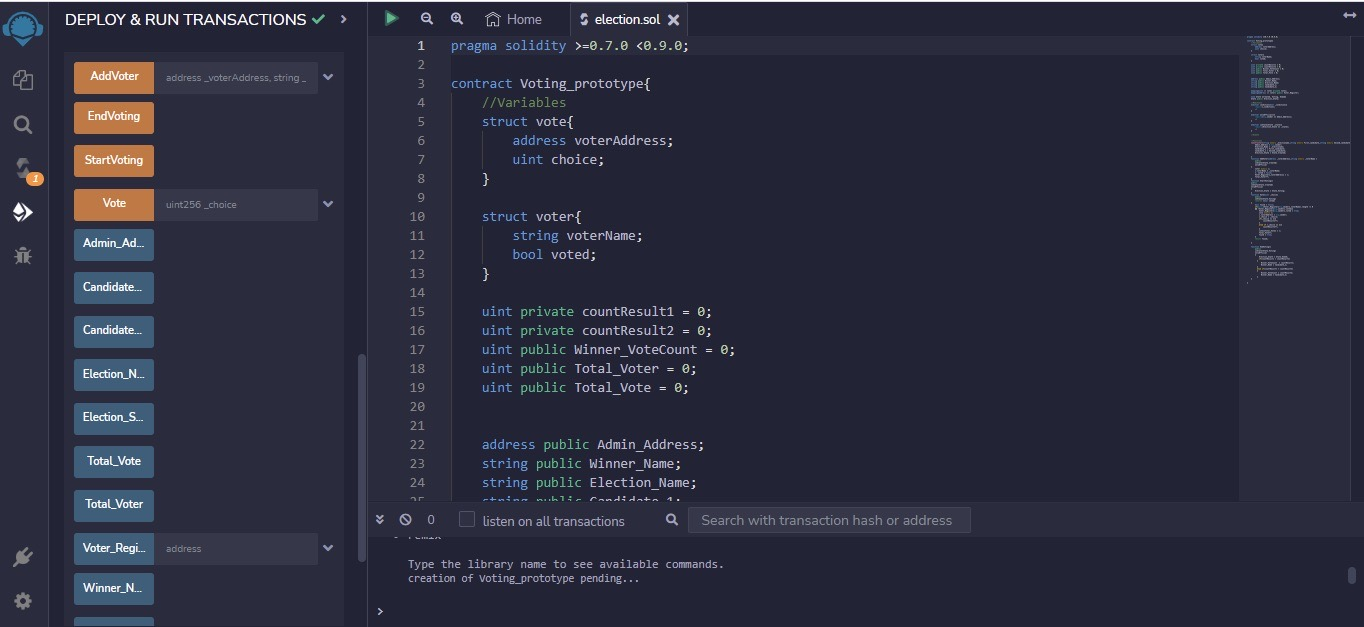
\includegraphics[scale=0.25]{images/SmartContractOutput.jpeg}
             %    \textit{\caption{Smart Contract Section..}}
               
            %  \label{fig:Activity Diagram 1}
    %   \end{figure}

%\listoffigures  List of figures%

\chapter{References}
       
       [1]	J. Chai, “Blockchain based voting system with Ethereum Blockchain,” Undergraduate, The Ohio State University, 2020.\\
       
[2]	R. Taş and Ö. Ö. Tanrıöver, “A Systematic Review of Challenges and Opportunities of Blockchain for E-Voting,” Symmetry, vol. 12, no. 8. p. 1328, 2020. doi: 10.3390/sym12081328.\\

[3]	F. Fusco, M. I. Lunesu, F. E. Pani, and A. Pinna, “Crypto-voting, a Blockchain based e-Voting System,” Proceedings of the 10th International Joint Conference on Knowledge Discovery, Knowledge Engineering and Knowledge Management. 2018. doi: 10.5220/0006962102230227.\\

[4]	K. M. Khan, J. Arshad, and M. M. Khan, “Secure Digital Voting System Based on Blockchain Technology,” Research Anthology on Blockchain Technology in Business, Healthcare, Education, and Government. pp. 1280–1290, 2021. doi: 10.4018/978-1-7998-5351-0.ch071.\\

[5]	U. Jafar, M. J. A. Aziz, and Z. Shukur, “Blockchain for Electronic Voting System-Review and Open Research Challenges,” Sensors , vol. 21, no. 17, Aug. 2021, doi: 10.3390/s21175874.\\

[6]	“An AI-driven and blockchain-secure electoral process,” TheCable, Jun. 07, 2022. https://www.thecable.ng/an-ai-driven-and-blockchain-secure-electoral-process (accessed Jun. 11, 2022).\\

[7]	“About Us —,” BallotReady. https://about.ballotready.org/about-us (accessed Jun. 11, 2022).\\

[8]	“Voatz,” Aug. 29, 2019. https://en.wikipedia.org/wiki/Voatz (accessed Jun. 11, 2022).\\

[9]	“Blockchain Voting: The End To End Process,” Follow My Vote, Dec. 01, 2014. https://followmyvote.com/blockchain-voting-the-end-to-end-process/ (accessed Jun. 11, 2022).\\



%[10]	Fri\ð rik Þ. Hj\á lmarsson, Gunnlaugur K. Hrei\ð arsson, Mohammad Hamdaqa, G\í sli Hj\á lmt\ý sson, “Blockchain-Based E-Voting System,” 2018 IEEE 11th International Conference on Cloud Computing (CLOUD), 2018, doi: 10.1109/CLOUD.2018.00151.

[11]	Q. Zhang, B. Xu, H. Jing, S. Zhang, and Z. Zheng, “Ques-Chain: An Ethereum Based E-Voting System,” 9th International Conference on Computer Science and Information Technology (CCSIT 2019). 2019. doi: 10.5121/csit.2019.90803.\\

[12]	A. M. Al-madani, A. T. Gaikwad, V. Mahale, and Z. A. T. Ahmed, “Decentralized E-voting system based on Smart Contract by using Blockchain Technology,” 2020 International Conference on Smart Innovations in Design, Environment, Management, Planning and Computing (ICSIDEMPC). 2020. doi: 10.1109/icsidempc49020.2020.9299581.\\

[13]	T. Contributor, “use case diagram (UML use case diagram),” www.techtarget.com, Jul. 2020. https://www.techtarget.com/whatis/definition/use-case-diagram (accessed Jun. 2022).\\

[14]	“Levels in data flow diagrams (DFD),” GeeksforGeeks, Mar. 18, 2019. https://www.geeksforgeeks.org/levels-in-data-flow-diagrams-dfd/ (accessed Jun. 11, 2022).\\

%[15]	“SDLC - Overview.” https://www.tutorialspoint.com/sdlc/sdlc_overview.htm (accessed Jun. 10, 2022).

[15] ''SDLC - Overview"(\href{ https://www.tutorialspoint.com/sdlc/sdlc_overview.htm})%{Something  Linky}%(accessed Jun.10,2022).


\end{document}
